\documentclass[letterpaper,12pt]{article}
\usepackage[a4paper]{geometry}
\usepackage{amsmath, amssymb, amsthm,graphicx}
\usepackage{fancyhdr}
\pagestyle{fancy}
\title{\textbf{Applications of the Singular Value Decomposition}}
\author{Justin Hood}
\date{\today}


\newcommand{\Z}{\mathbb{Z}}
\newcommand{\Q}{\mathbb{Q}}
\newcommand{\R}{\mathbb{R}}
\newcommand{\C}{\mathbb{C}}
\newtheorem{lem}{Lemma}

\begin{document}
\maketitle
\newpage
\begin{abstract}
The Singular Value Decomposition is a powerful tool at the disposal of modern mathematicians. By breaking down a matrix $A$ into its components $A=USV^T$, we are able to do different analysis than we would be able to with the matrix itself. In this project, we consider two such examples, one analyzing the voting patterns of Senators through various sessions of congress, and the other concerning image processing and storage. In each of these two different methods, the SVD is used in a different way, lending to the strength of this decomposition. Not only can we use fewer terms of the decomposed matrices to approximate the original matrix, the values of the eigenvector output are also quite informative, as we will see later on. Overall, we will see that the SVD is an invaluable tool in data analysis, and now that there exists efficient methods for computing it on large data matrices, it has become an even more accessible tool as well.
\end{abstract}
\newpage

\tableofcontents
\newpage

\section{Introduction}
To begin our analysis, we shall begin by defining the SVD, and how it is computed.
\subsection{SVD}
For a matrix $A$ in $\R^{m\times n}$, there exists a factorization,
\[A=USV^T\]
These matrices may be computed, where $U\in \R^{m\times m}$ and $V\in \R^{n\times n}$ are orthogonal matrices, and $S\in \R^{m\times n}$ is a diagonal matrix of the square roots of the non-zero eigenvalues of $A$. These ``singular values" are computed from the square matrices $AA^T$ and $A^TA$ and then taking the positive root. It can be shown that for a any matrix $A$, the SVD exists, which is a powerful piece of information at our disposal.\cite{Extra}\\
With this definition of the SVD, it is natural to progress to questioning how it is computed. So, we consider the computational process. First, we compute the eigenvalues and eigenvectors of the symmetric matrix, $AA^T$. Then, the singular values are computed and ordered in descending order starting with the largest singular value. The columns of our eigenvector matrix are permuted accordingly, so that they match their associated singular value. This new eigenvector matrix forms our $U$ matrix. This process is repeated for the matrix $A^TA$, which by definition will have the same non-zero singular values as $AA^T$. The associated eigenvectors for this matrix, when ordered as before form the $V$ matrix. Finally, the singular values are placed on the diagonal of a matrix and padded with zeros to match the dimensions of the $U$ and $V^T$ matrix for multiplication purposes. We note here, that the computed eigenvectors are unique up to a sign, and so computer output may require some modification to reproduce the original matrix.\cite{SVDHowTo}\\
It is important to note, however, that for a naturally symmetric matrix, $A=A^T$, many of these computations can be ignored, as we only need the eigenvalues and vectors of the $A$ matrix. An example of this is contained in the attached notebook.
\subsection{Truncated SVD}
Now that we have defined the SVD and how it is computed, we can also consider the following,
\[A=USV^T=\sum\sigma_iu_iv^T_i\]
I.e., we may write the full SVD as the sum of the product of the singular values, and paired columns and rows of the $U$ and $V$ matrices. As we might expect, we can write a truncated form of this sum as,
\[A_k = \sum_{i=1}^k\sigma_iu_iv^T_i\]
This sum will not be an exact approximation, but for large data sets, we may often be able to fairly accurately represent the data with less terms of the sum, thereby saving us a great deal with computational space and time. We will explore this idea again later on with our image processing example.\cite{Extra}
\subsection{SVD Computation in Python}
To start this project, we consider how the SVD could be computed in Python using the NumPy library. We will use the NumPy library as its ability to do matrix computations is ideal for our purposes. From before, we consider the pseudo code below for computing the SVD.
\begin{verbatim}
Test if matrix is symmetric (A=A^T)
If(Symmetric):
    D,V = np.linalg.eig(A) # Get the eigenvalues and vectors No need for AA^T
    Order Eigenvalues
    return V,s,V
	
Else:
    D,V = np.linalg.eig(np.dot(A.T,A)) # Get the eigenvalues and vectors
    D=sqrt(D) #Singular values
    s=D[np.flip(np.argsort(D))] #Sort the singular values by magnitude
    V=V[:,np.flip(np.argsort(D))] #Move the columns of the V matrix to match
    U = A.dot(V)/s 
    #Note VV^T=I So, AV=US, and S is just a diagonal entry of values.
return U,s,V Here are the matrices we want.
\end{verbatim}
This pseudocode is enacted in the associated file ``Final SVD.ipynb".
\section{Voting Application}
Now that we have looked at the SVD and computations associated with it, we consider our first application. For this application, we will be looking at Senate voting data over a number of sessions of Congress. We will create a matrix of votes based on the votes of each sitting Senator, and then perform a SVD on the data. From the $U$ $s$ and $V$ matrices that the SVD produces, we will interpret the output, and plot the data.
\subsection{Process}
To begin the analysis of the Senate voting data, we must first choose the data to use in our analysis. The \textit{senate.gov} website contains roll call voting data from the Senate starting with the 101st congress in 1989, through current day votes. Because of the complexity in gathering the data from this site, we will look at the data from a subset of congressional sessions, specifically sessions $(101,104,107,110,113)$. These sessions of congress range from 1989 through 2014, and should serve to provide a time sensitive analysis of the voting patterns of Senators by party.  With the sessions decided upon, we now consider how to represent the voting data. Using the ideas set forth in the \textit{The Extraordinary SVD} paper, we consider the following partition of the votes,
\[\begin{cases}
1 & \text{If ``Yea"}\\
0 & \text{If ``Not Voting"}\\
-1 & \text{If ``Nay"}
\end{cases}\]
As such, we are able to numerically represent each persons votes into a vector. Once the data has been gathered, these vectors are relatively simple to work with, they are easily combined into a larger master voting matrix for our SVD analysis.
\subsubsection{Senator Class}
In order to retain as much information about each Senator's voting history as possible, we create a custom python class object ``Senator" that contains several key pieces of information about the Senator, like their name, party affiliation, and a vector of their votes for that session of congress. Importing this class into the main notebook, we are able to parse each of the vote outputs and create a vector of Senator class objects that all had their unique voting history. From there is is merely a matter of combining each of the voting vectors into an $n\times m$ matrix, with $n=$ the number of senators (In case of special election $n> 100$) and $m=$ the number of bills voted upon in that session. As a note, for this project, we are only gathering the data on votes that specifically deal with bills. Other votes, such as confirmations and clotures are ignored to both simplify the gathering process as well as to avoid artificial shifts in the data. Votes like confirmations tend to be quite politicized on a scale that far exceeds normal bill voting procedure, so these votes could represent a more severe dichotomy than is the norm in the results.
\subsubsection{SVD of the Voting Matrix}
Now that the data has been coerced into a more workable form, we are looking at a matrix of the form,
\[Votes=\begin{bmatrix}
1 & -1 & 0 & \ldots\\
\vdots & \vdots & \vdots & \ddots
\end{bmatrix} \]
Where the entries of each row correspond to a particular Senators votes over the session. With this matrix, we may now use NumPy to perform a SVD of the data. With $U$, $s$ and $V$ defined by the SVD call, we consider how much of the data is represented by each of the singular values. Taking a note from the ideas of Principle Component Analysis, we look at a sort of Scree chart of the singular values to see how well they represent our data.
\begin{center}
\includegraphics[scale=.75]{votescree.png}
\end{center}
Looking at the data in this way, we see that the first two singular values of the decomposition account for a much larger proportion of the data than the rest of the values. As such, we might be interested in looking at the values of the $U$ matrix for the first two columns. It is known that for voting data like the above, that the first column of the $U$ matrix corresponds to a ``Partisan" coordinate, a measure of party affiliation of the senator, and that the second column represents a ``bipartisan" coordinate, a measure of how often the congressman votes with the majority.\cite{Extra} As such, plotting these values against each other will provide us a way of seeing natural clusters within the voting data, and perhaps reveal hidden patterns in the data. The following pseudo code explains our process in Python for constructing the plots below.
\subsubsection{Vote Computations Pseudo Code}
\begin{verbatim}
Get initial Senate session URL
From this URL find the curls for each "Bill" vote, store in list
For first vote:
    Parse vote results and create new senator class object with initial votes (-1,0,1)
For remaining votes:
    Parse vote results and append new vote (-1,0,1) by Senator
Stack all vote vectors into matrix
U,s,V = np.svd(VoteMatrix)
Plot(U[:,0], U[:,1]) with points representative of party
Repeat for all Senate sessions
\end{verbatim}
\subsection{Results}
Applying the above process to the senate voting data from the $107th$ congress, we obtain the following plots of,
\begin{center}
\includegraphics[scale=.5]{107th1.png}
\includegraphics[scale=.5]{107th2.png}
\end{center}
We see from the images that the Democrats and Republicans of the 107th Senate do tend to cluster with their respective parties, and that interestingly enough the Senators who are Independents have approximately zero partisan scores. This shows that these parties tend to vote alongside their compatriots, with the Independents being neutral to party bias, as we would expect in an ``ideal" situation. We also note that the bipartisan coordinate for all of the Senators is positive, which also implies that regardless of party, many of the roll call votes that were taken involved a majority of both parties to vote in the same way, an interesting point to note as well. We also see that there are more points within the second session that cluster around the 0 mark for the partisan coordinate than the first session. These points correspond to Senators who do not necessarily vote strictly along party lines.\\
Now, we consider looking at several plots of the various sessions in time order, to see if we notice a drift to our current political climate of party isolation.
\begin{center}
\includegraphics[scale=.25]{101st1.png}
\includegraphics[scale=.25]{104th1.png}
\includegraphics[scale=.25]{107th1.png}
\includegraphics[scale=.25]{110th1.png}
\includegraphics[scale=.25]{113th2.png}
\end{center}
We see that for the 101st (1989) congress, there is significantly more partisan mixing than in the later years. We also see that for the 104th session (1994/95), that there is a strong split between the two parties both in terms of partisanship and bipartisanship. This could be due in part to the political climate of the time, coming out of the Gulf and Cold Wars, there was a significant division in the parties of congress regarding how the conflict was handled. We see that as we move on chronologically, the parties begin to slightly drift back towards each other, while retaining their isolated clustering. We do see interestingly that as time progresses, one of the parties bipartisan coordinates begins to drift into the negatives, which implies that the parties are not as cooperative in terms of overall votes. This mirrors what we might expect from our current climate, with the parties in congress actively voting against each other.
\section{Image Processing Application}
Seeing how the $U$ and $V$ vectors contain information about the overall nature of the matrix is one interesting aspect of the SVD, but there are other applications of the SVD that do not necessarily require looking deeper into the columns of the component matrices. Looking back to before when we defined our truncated sum, we see that a given matrix $A$ can be partially represented by the sum of the first $k$ terms of the product. As such, we can store the information in a matrix to a degree of accuracy using $k$ columns of $U$ and $k$ rows of the $V$ matrix, which only requires $k(m+n+1)$ values. For large matrices, this can be a dramatic reduction in data needed to store, which can be very helpful in many settings. For example, consider how an image can be represented in a computer.
\subsection{Python Representation}
In Python and various other languages, images are represented by matrices of values that correspond to the red, blue, and green color strengths for each pixel. With these numeric values, transformations like the FFT can be computed to change or study the image. Here we consider representing images with less data than the original matrix of color values. To begin, I took a picture of my cats to use as an example.
\begin{center}
\includegraphics[scale=.08]{RasandThea.png}\\
My cats Ra's (Lower) and Thea (Upper). Named after the DC comics characters Ra's Al Guhl and Thea Queen
\end{center}
Using the Python Imaging Library (PIL), we load this image into our notebook and convert it into a NumPy array. Getting the shape of this array, we find that this image is $4032\times 3024$ pixels. As such, our NumPy array will have dimensions $4032\times 3024\times 3$, a separate $4032\times 3024$ array for each of our RGB color values.
\subsubsection{Grey Scale}
For our first test, we will consider the matrix representation of the image in a grey scale form. To a computer, grey is represented as the same value for each of the colors. I.e. a grey pixel is one where $R=B=G$. Usually, when I have encountered the grey scaling transformation, it is done as a true average of the three color values. But, the PIL uses the equation,\cite{PIL}
\[L=R(299/1000)+G(587/1000)+B(114/1000)\]
to scale the colors. This is not of great import, but is worth knowing to replicate the result. Once the image has been scaled by the above function, we arrive at the image below,
\begin{center}
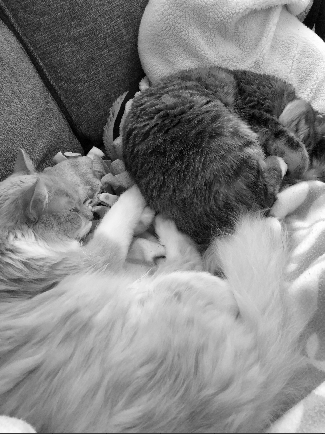
\includegraphics[scale=.75]{RasandTheaGrey.png}
\end{center}
Now, we apply the SVD to the grey color matrix and compute an approximation to the original image using the first $k$ terms of the series representation.
\subsubsection{Grey Scale Results}
Below are the first few approximations to the image using $k=5,10,50$ respectively,
\begin{center}
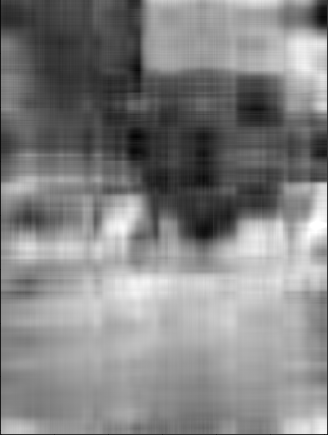
\includegraphics[scale=.4]{grey5.png}
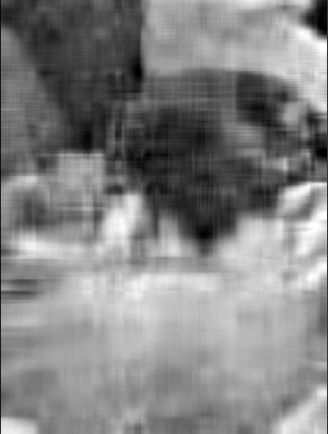
\includegraphics[scale=.4]{grey10.png}
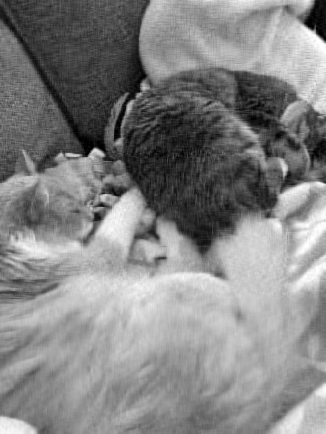
\includegraphics[scale=.4]{grey50.png}
\end{center}
We see that for the first image, $k=5$, that the image is a very poor approximation of the original. You can make out only a fraction of the shapes and color scales of the original image. The $k=10$ approximation is significantly better than the original, but still quite blurry. Finally, we see that with $k=50$, we actually get a good approximation to the true image. Moving forward, we consider a $k=100$ approximation,
\begin{center}
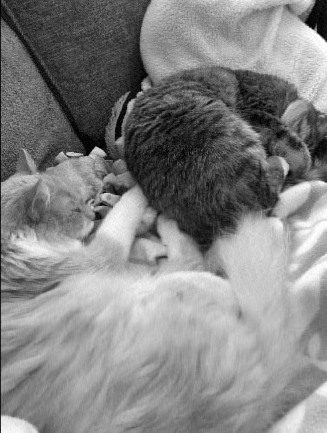
\includegraphics[scale=.6]{grey100.png}
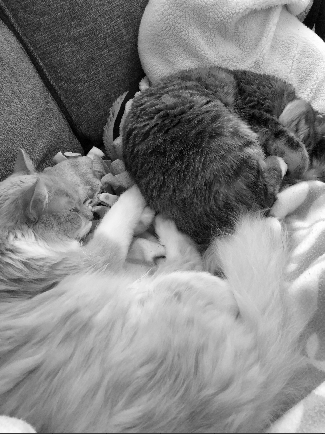
\includegraphics[scale=.6]{RasandTheaGrey.png}
\end{center}
We see that the $k=100$ approximation (left) and the true image (right) are practically indiscernible from each other. So, we see that the image is well represented by $100$ terms of the series. To see how good of a reduction in points this is, we consider the number of values required to store the first $100$ vectors of $U$ and $V$ as well as $100$ singular values versus the total number of points in the image.
\[S_{100}=\frac{100(4032+3024+1)}{4032(3024)}=5.79\%\]
So, we see that we can encode a photo realistic approximation to our image using less than 6\% of the original number of points. This is a huge savings, and is worth noting that other large complex data sets can be encoded this way as well.
\subsection{Color Approximations}
As before, we consider how we might compute a truncated sum to approximate the color image. Given that we have the color image as 3 arrays of color values, we consider the approximation below,
\begin{align*}
r &\approx kth\ approximation\ of\ R\ Matrix\\
b &\approx kth\ approximation\ of\ B\ Matrix\\
g &\approx kth\ approximation\ of\ G\ Matrix\\
Image &= [r,b,g]
\end{align*}
So, with this implementation in mind, we compute the following $k=1$ approximation to the color image,
\begin{center}

\includegraphics[scale=.6]{col1.png}
\end{center}
We see here that the rows of the image are dominated by the average color value, so that the image appears to be a gradient from dark to light. This gradient matches the original picture, as Thea has dark fur, whereas Ra's has lighter tan fur. As before, we also compute the $k=5,50,100$ approximations,
\begin{center}
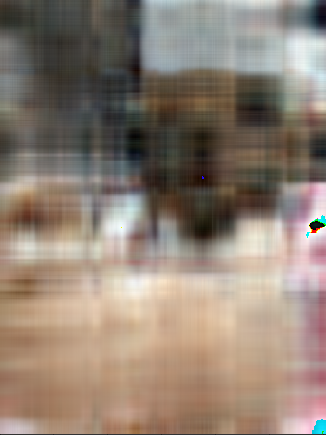
\includegraphics[scale=.4]{col5.png}
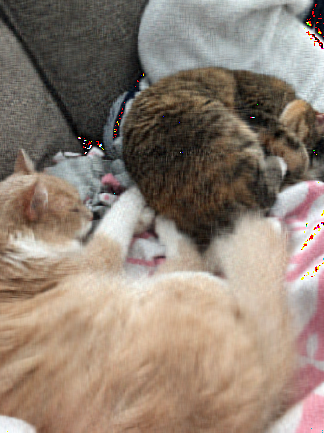
\includegraphics[scale=.4]{col50.png}
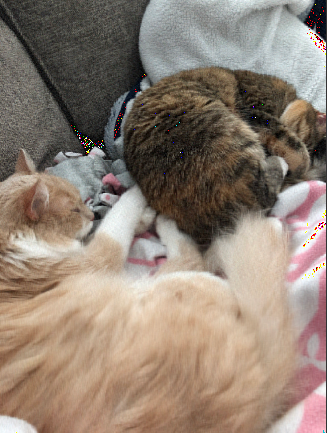
\includegraphics[scale=.4]{col100.png}
\end{center}
We note here that the image sharpens as before, with the last image being an almost perfect replication of the original, save a few random points of color. As we increase $k$, we notice these basins of random color move around and change in size. Thinking about how the computer interprets color, we know that large values of each color are considered black. So, these are likely points in each color matrix that are converging to their large values faster than the others, so we see a sharp color as opposed to the black it will eventually become as the series continues.\\
As before, we might consider how much of a reduction in space this is, specifically for the $k=100$ case.
\[S_{100}=\frac{100(4032+3024+1)(3)}{4032(3024)(3)}=5.79\%\]
We see that this is the same value as before, as we have merely increased the dimension of the data by 3 in both cases. As such, we require the same proportion of data to encode the image, but this amount is 3 times what it was before.
\section{Conclusions}
As we have seen, the SVD has many applications to the fields of mathematics and data science. By being able to represent a matrix in this broken down form, new information about the data can be gleaned. In addition to this, with the continual improvements in computing power and optimized algorithms that are readily becoming more available to the general populus, SVD analysis and its applications are becoming increasingly important and relevant in innumerable ways.
\subsection{Extensions}
After exploring the applications of the SVD as we have above, we begin to get a sense of what the SVD is capable of, and how it could be potentially used in other ways. Looking first at the vote analysis that we did, we see that it takes a principal component analysis flavor from statistics. In this way, we begin to consider how many different data sets that can be analyzed in this way. Given that data from the internet is fairly accessible with basic Python libraries, more and more data is accessible to the modern student or researcher. In addition to looking at the hidden structures within the data, we also see that there is a capability for prediction of future results using the SVD. Because we can predict how a Senator will vote based on party lines and bipartisanship, given information about a given bill will allow us to predict how the vote will occur. This type of analysis is much sought after, and accuracy and speed at this computation is quite valuable. So, we see that the SVD is valuable in almost innumerable ways, and even in ways that have not been thought of yet.
\newpage
\begin{thebibliography}{9}
\bibitem{Extra}
Martin C. D.,  Porter M. A.. The extraordinary SVD, \textit{Am. Math. Monthly} , 2012, vol. 119 (pg. 838-851)
\bibitem{SVDHowTo}
Web.mit.edu. (2019). \textit{Singular Value Decomposition (SVD) tutorial}. [online] Available at: http://web.mit.edu/be.400/www/SVD/Singular\_ Value\_ Decomposition.htm [Accessed 10 May 2019].
\bibitem{PIL}
Pillow.readthedocs.io. (2019). \textit{Image Module} - \textit{Pillow (PIL Fork) 3.1.2 documentation.} [online] Available at: https://pillow.readthedocs.io/en/3.1.x/reference/Image.html [Accessed 10 May 2019].
\bibitem{Network}
Porter, Mason A., Mucha, Peter J., Newman, M. E. J., and Warmbrand, Casey M. 2005. A network analysis of committees in the U.S. House of Representatives. \textit{Proceedings of the National Academy of Sciences of the United States of America} \textbf{102}: 7057–62.
\end{thebibliography}
\end{document}
